
\documentclass[11pt]{article}
\usepackage[hmargin=1in,vmargin=1in]{geometry}
\usepackage{xcolor}
\usepackage{mdframed}
\newmdenv[linecolor=blue,backgroundcolor=blue!10]{mybox}
\usepackage{tikz}
\usepackage{enumitem}
\usepackage{amsmath,amssymb,amsfonts,url,sectsty,framed,tcolorbox,framed}
\newcommand{\pf}{{\bf Proof: }}
\newtheorem{theorem}{Theorem}
\newtheorem{lemma}{Lemma}
\newtheorem{proposition}{Proposition}
\newtheorem{definition}{Definition}
\newtheorem{remark}{Remark}
\newcommand{\qed}{\hfill \rule{2mm}{2mm}}
\usepackage{enumitem}



\begin{document}
%%%%%%%%%%%%%%%%%%%%%%%%%%%%%%%%%%%%%%%%%%%%%%%%%%%%%%%%%%%%%%%%%%%%%
\noindent
\rule{\textwidth}{1pt}
\begin{center}
{\bf [CS304] Introduction to Cryptography and Network Security}
\end{center}
Course Instructor: Dr. Dibyendu Roy \hfill Winter 2023-2024\\
Scribed by: Manas Jitendrakumar Ingle (202151086) \hfill Lecture 1,2 (Weak 1)
\\
\rule{\textwidth}{1pt}
%%%%%%%%%%%%%%%%%%%%%%%%%%%%%%%%%%%%%%%%%%%%%%%%%%%%%%%%%%%
%write here

\section*{Data Encryption Standard}

Flowchart for encrypting block of text using DES:
\begin{center}
    \tikzset{every picture/.style={line width=0.75pt}} 
    
    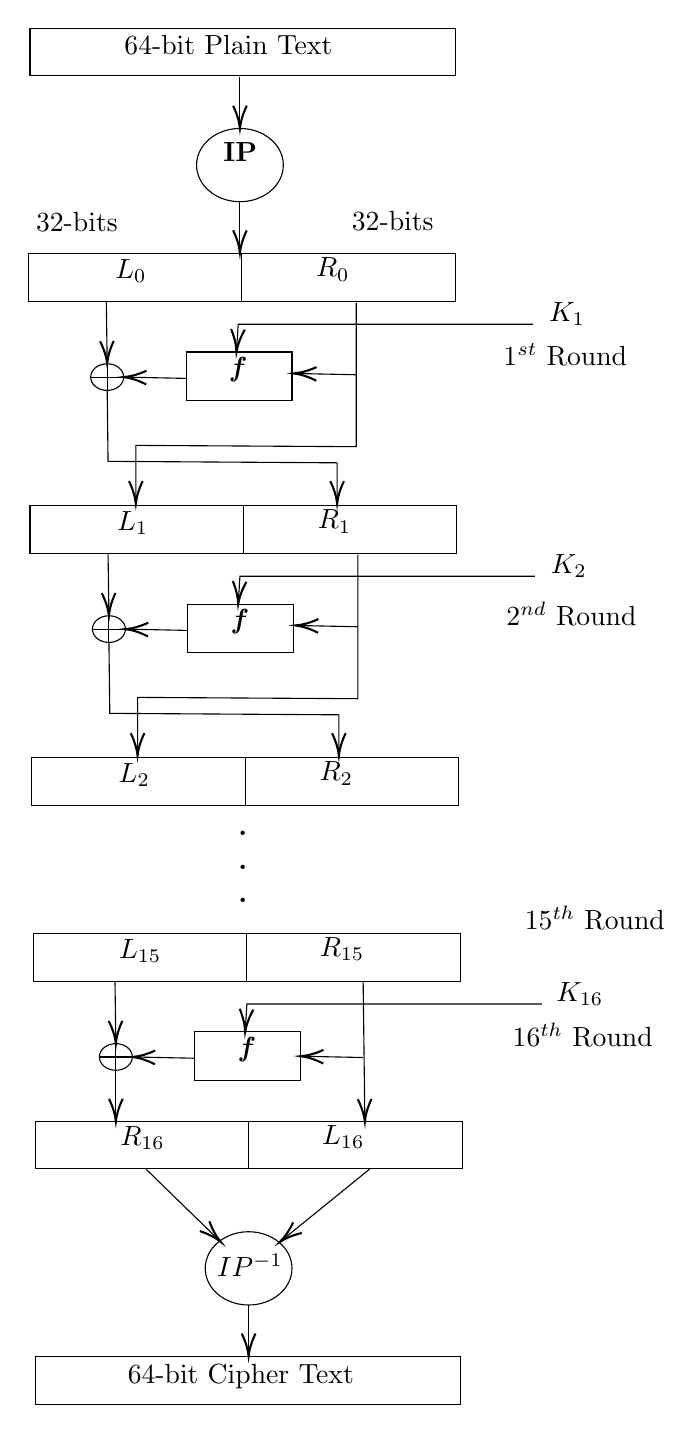
\begin{tikzpicture}[x=0.75pt,y=0.75pt,yscale=-1,xscale=1]
    
    \draw   (192.84,35) -- (397.67,35) -- (397.67,57.87) -- (192.84,57.87) -- cycle ; 
    \draw    (294,58.58) -- (294,81.28) ;
    \draw [shift={(294,83.28)}, rotate = 270] [color={rgb, 255:red, 0; green, 0; blue, 0 }  ][line width=0.75]    (10.93,-3.29) .. controls (6.95,-1.4) and (3.31,-0.3) .. (0,0) .. controls (3.31,0.3) and (6.95,1.4) .. (10.93,3.29)   ; 
    \draw   (273.1,100.93) .. controls (273.1,91.19) and (282.46,83.28) .. (294,83.28) .. controls (305.54,83.28) and (314.9,91.19) .. (314.9,100.93) .. controls (314.9,110.68) and (305.54,118.58) .. (294,118.58) .. controls (282.46,118.58) and (273.1,110.68) .. (273.1,100.93) -- cycle ;
    \draw   (192,143.71) -- (294.84,143.71) -- (294.84,166.58) -- (192,166.58) -- cycle ;
    \draw    (294,118.58) -- (294,141.29) ;
    \draw [shift={(294,143.29)}, rotate = 270] [color={rgb, 255:red, 0; green, 0; blue, 0 }  ][line width=0.75]    (10.93,-3.29) .. controls (6.95,-1.4) and (3.31,-0.3) .. (0,0) .. controls (3.31,0.3) and (6.95,1.4) .. (10.93,3.29)   ;
    \draw   (294.84,143.71) -- (397.67,143.71) -- (397.67,166.58) -- (294.84,166.58) -- cycle ;
    \draw   (268.08,191.01) -- (319.08,191.01) -- (319.08,214.44) -- (268.08,214.44) -- cycle ; 
    \draw   (222.1,203.08) .. controls (222.1,199.53) and (225.65,196.66) .. (230.04,196.66) .. controls (234.43,196.66) and (237.98,199.53) .. (237.98,203.08) .. controls (237.98,206.63) and (234.43,209.5) .. (230.04,209.5) .. controls (225.65,209.5) and (222.1,206.63) .. (222.1,203.08) -- cycle ; \draw   (222.1,203.08) -- (237.98,203.08) ; \draw   (230.04,196.66) -- (230.04,209.5) ;
    \draw    (350.02,167.29) -- (350.02,236.61) -- (253.87,236.04) -- (243.84,235.98) -- (243.84,262.14) ;
    \draw [shift={(243.84,264.14)}, rotate = 270] [color={rgb, 255:red, 0; green, 0; blue, 0 }  ][line width=0.75]    (10.93,-3.29) .. controls (6.95,-1.4) and (3.31,-0.3) .. (0,0) .. controls (3.31,0.3) and (6.95,1.4) .. (10.93,3.29)   ;
    \draw   (192.84,265.13) -- (295.67,265.13) -- (295.67,288) -- (192.84,288) -- cycle ;
    \draw   (295.67,265.13) -- (398.51,265.13) -- (398.51,288) -- (295.67,288) -- cycle ;
    \draw    (350.02,201.95) -- (321.92,201.36) ;
    \draw [shift={(319.92,201.31)}, rotate = 1.21] [color={rgb, 255:red, 0; green, 0; blue, 0 }  ][line width=0.75]    (10.93,-3.29) .. controls (6.95,-1.4) and (3.31,-0.3) .. (0,0) .. controls (3.31,0.3) and (6.95,1.4) .. (10.93,3.29)   ;
    \draw    (268.08,203.71) -- (239.98,203.12) ;
    \draw [shift={(237.98,203.08)}, rotate = 1.21] [color={rgb, 255:red, 0; green, 0; blue, 0 }  ][line width=0.75]    (10.93,-3.29) .. controls (6.95,-1.4) and (3.31,-0.3) .. (0,0) .. controls (3.31,0.3) and (6.95,1.4) .. (10.93,3.29)   ;
    \draw    (229.62,166.58) -- (230.01,194.66) ;
    \draw [shift={(230.04,196.66)}, rotate = 269.2] [color={rgb, 255:red, 0; green, 0; blue, 0 }  ][line width=0.75]    (10.93,-3.29) .. controls (6.95,-1.4) and (3.31,-0.3) .. (0,0) .. controls (3.31,0.3) and (6.95,1.4) .. (10.93,3.29)   ; 
    \draw    (230.04,209.5) -- (230.46,243.67) -- (340.82,244.38) -- (340.82,262.14) ;
    \draw [shift={(340.82,264.14)}, rotate = 270] [color={rgb, 255:red, 0; green, 0; blue, 0 }  ][line width=0.75]    (10.93,-3.29) .. controls (6.95,-1.4) and (3.31,-0.3) .. (0,0) .. controls (3.31,0.3) and (6.95,1.4) .. (10.93,3.29)   ;
    \draw    (435.3,177.6) -- (293.16,177.6) -- (292.45,189.01) ;
    \draw [shift={(292.33,191.01)}, rotate = 273.57] [color={rgb, 255:red, 0; green, 0; blue, 0 }  ][line width=0.75]    (10.93,-3.29) .. controls (6.95,-1.4) and (3.31,-0.3) .. (0,0) .. controls (3.31,0.3) and (6.95,1.4) .. (10.93,3.29)   ;
    \draw   (268.92,312.43) -- (319.92,312.43) -- (319.92,335.86) -- (268.92,335.86) -- cycle ; 
    \draw   (222.93,324.5) .. controls (222.93,320.95) and (226.49,318.07) .. (230.88,318.07) .. controls (235.26,318.07) and (238.82,320.95) .. (238.82,324.5) .. controls (238.82,328.05) and (235.26,330.92) .. (230.88,330.92) .. controls (226.49,330.92) and (222.93,328.05) .. (222.93,324.5) -- cycle ; \draw   (222.93,324.5) -- (238.82,324.5) ; \draw   (230.88,318.07) -- (230.88,330.92) ;
    \draw    (350.85,288.71) -- (350.85,358.03) -- (254.71,357.46) -- (244.67,357.4) -- (244.67,383.56) ;
    \draw [shift={(244.67,385.56)}, rotate = 270] [color={rgb, 255:red, 0; green, 0; blue, 0 }  ][line width=0.75]    (10.93,-3.29) .. controls (6.95,-1.4) and (3.31,-0.3) .. (0,0) .. controls (3.31,0.3) and (6.95,1.4) .. (10.93,3.29)   ; 
    \draw   (193.67,386.55) -- (296.51,386.55) -- (296.51,409.42) -- (193.67,409.42) -- cycle ;
    \draw   (296.51,386.55) -- (399.35,386.55) -- (399.35,409.42) -- (296.51,409.42) -- cycle ;
    \draw    (350.85,323.37) -- (322.75,322.78) ;
    \draw [shift={(320.76,322.73)}, rotate = 1.21] [color={rgb, 255:red, 0; green, 0; blue, 0 }  ][line width=0.75]    (10.93,-3.29) .. controls (6.95,-1.4) and (3.31,-0.3) .. (0,0) .. controls (3.31,0.3) and (6.95,1.4) .. (10.93,3.29)   ; 
    \draw    (268.92,325.13) -- (240.82,324.54) ;
    \draw [shift={(238.82,324.5)}, rotate = 1.21] [color={rgb, 255:red, 0; green, 0; blue, 0 }  ][line width=0.75]    (10.93,-3.29) .. controls (6.95,-1.4) and (3.31,-0.3) .. (0,0) .. controls (3.31,0.3) and (6.95,1.4) .. (10.93,3.29)   ;
    \draw    (230.46,288) -- (230.85,316.07) ;
    \draw [shift={(230.88,318.07)}, rotate = 269.2] [color={rgb, 255:red, 0; green, 0; blue, 0 }  ][line width=0.75]    (10.93,-3.29) .. controls (6.95,-1.4) and (3.31,-0.3) .. (0,0) .. controls (3.31,0.3) and (6.95,1.4) .. (10.93,3.29)   ;
    \draw    (230.88,330.92) -- (231.3,365.09) -- (341.66,365.79) -- (341.66,383.56) ;
    \draw [shift={(341.66,385.56)}, rotate = 270] [color={rgb, 255:red, 0; green, 0; blue, 0 }  ][line width=0.75]    (10.93,-3.29) .. controls (6.95,-1.4) and (3.31,-0.3) .. (0,0) .. controls (3.31,0.3) and (6.95,1.4) .. (10.93,3.29)   ;
    \draw    (436.13,299.01) -- (294,299.01) -- (293.29,310.43) ;
    \draw [shift={(293.16,312.43)}, rotate = 273.57] [color={rgb, 255:red, 0; green, 0; blue, 0 }  ][line width=0.75]    (10.93,-3.29) .. controls (6.95,-1.4) and (3.31,-0.3) .. (0,0) .. controls (3.31,0.3) and (6.95,1.4) .. (10.93,3.29)   ;
    \draw   (194.51,471.26) -- (297.35,471.26) -- (297.35,494.13) -- (194.51,494.13) -- cycle ; 
    \draw   (297.35,471.26) -- (400.18,471.26) -- (400.18,494.13) -- (297.35,494.13) -- cycle ;
    \draw   (272.26,518.56) -- (323.26,518.56) -- (323.26,541.99) -- (272.26,541.99) -- cycle ;
    \draw   (226.28,530.63) .. controls (226.28,527.08) and (229.84,524.2) .. (234.22,524.2) .. controls (238.61,524.2) and (242.16,527.08) .. (242.16,530.63) .. controls (242.16,534.17) and (238.61,537.05) .. (234.22,537.05) .. controls (229.84,537.05) and (226.28,534.17) .. (226.28,530.63) -- cycle ; \draw   (226.28,530.63) -- (242.16,530.63) ; \draw   (234.22,524.2) -- (234.22,537.05) ;
    \draw    (233.8,494.13) -- (234.19,522.2) ;
    \draw [shift={(234.22,524.2)}, rotate = 269.2] [color={rgb, 255:red, 0; green, 0; blue, 0 }  ][line width=0.75]    (10.93,-3.29) .. controls (6.95,-1.4) and (3.31,-0.3) .. (0,0) .. controls (3.31,0.3) and (6.95,1.4) .. (10.93,3.29)   ;
    \draw    (439.48,505.14) -- (297.35,505.14) -- (296.63,516.56) ;
    \draw [shift={(296.51,518.56)}, rotate = 273.57] [color={rgb, 255:red, 0; green, 0; blue, 0 }  ][line width=0.75]    (10.93,-3.29) .. controls (6.95,-1.4) and (3.31,-0.3) .. (0,0) .. controls (3.31,0.3) and (6.95,1.4) .. (10.93,3.29)   ;
    \draw   (195.34,561.62) -- (298.18,561.62) -- (298.18,584.49) -- (195.34,584.49) -- cycle ;
    \draw   (298.18,561.62) -- (401.02,561.62) -- (401.02,584.49) -- (298.18,584.49) -- cycle ;
    \draw    (353.36,530.91) -- (325.26,530.32) ;
    \draw [shift={(323.26,530.27)}, rotate = 1.21] [color={rgb, 255:red, 0; green, 0; blue, 0 }  ][line width=0.75]    (10.93,-3.29) .. controls (6.95,-1.4) and (3.31,-0.3) .. (0,0) .. controls (3.31,0.3) and (6.95,1.4) .. (10.93,3.29)   ;
    \draw    (353.36,494.13) -- (354.17,559.9) ;
    \draw [shift={(354.2,561.9)}, rotate = 269.29] [color={rgb, 255:red, 0; green, 0; blue, 0 }  ][line width=0.75]    (10.93,-3.29) .. controls (6.95,-1.4) and (3.31,-0.3) .. (0,0) .. controls (3.31,0.3) and (6.95,1.4) .. (10.93,3.29)   ;
    \draw    (234.22,537.05) -- (234.22,559.76) ;
    \draw [shift={(234.22,561.76)}, rotate = 270] [color={rgb, 255:red, 0; green, 0; blue, 0 }  ][line width=0.75]    (10.93,-3.29) .. controls (6.95,-1.4) and (3.31,-0.3) .. (0,0) .. controls (3.31,0.3) and (6.95,1.4) .. (10.93,3.29)   ;
    \draw   (277.28,632.49) .. controls (277.28,622.74) and (286.64,614.84) .. (298.18,614.84) .. controls (309.73,614.84) and (319.08,622.74) .. (319.08,632.49) .. controls (319.08,642.24) and (309.73,650.14) .. (298.18,650.14) .. controls (286.64,650.14) and (277.28,642.24) .. (277.28,632.49) -- cycle ; 
    \draw    (248.85,584.77) -- (283.37,618.39) ;
    \draw [shift={(284.8,619.78)}, rotate = 224.24] [color={rgb, 255:red, 0; green, 0; blue, 0 }  ][line width=0.75]    (10.93,-3.29) .. controls (6.95,-1.4) and (3.31,-0.3) .. (0,0) .. controls (3.31,0.3) and (6.95,1.4) .. (10.93,3.29)   ;
    \draw    (356.71,584.49) -- (314.78,618.52) ;
    \draw [shift={(313.23,619.78)}, rotate = 320.93] [color={rgb, 255:red, 0; green, 0; blue, 0 }  ][line width=0.75]    (10.93,-3.29) .. controls (6.95,-1.4) and (3.31,-0.3) .. (0,0) .. controls (3.31,0.3) and (6.95,1.4) .. (10.93,3.29)   ; 
    \draw    (298.18,650.14) -- (298.18,672.85) ;
    \draw [shift={(298.18,674.85)}, rotate = 270] [color={rgb, 255:red, 0; green, 0; blue, 0 }  ][line width=0.75]    (10.93,-3.29) .. controls (6.95,-1.4) and (3.31,-0.3) .. (0,0) .. controls (3.31,0.3) and (6.95,1.4) .. (10.93,3.29)   ;
    \draw   (195.34,675.13) -- (400.18,675.13) -- (400.18,698) -- (195.34,698) -- cycle ;
    \draw    (272.26,531.26) -- (244.16,530.67) ;
    \draw [shift={(242.16,530.63)}, rotate = 1.21] [color={rgb, 255:red, 0; green, 0; blue, 0 }  ][line width=0.75]    (10.93,-3.29) .. controls (6.95,-1.4) and (3.31,-0.3) .. (0,0) .. controls (3.31,0.3) and (6.95,1.4) .. (10.93,3.29)   ;
    
    \draw (237.08,37.29) node [anchor=north west][inner sep=0.75pt]   [align=left] {64-bit Plain Text};
    \draw (284.76,88.65) node [anchor=north west][inner sep=0.75pt]   [align=left] {\textbf{IP}};
    \draw (232.67,145.12) node [anchor=north west][inner sep=0.75pt]   [align=left] {$L_0$};
    \draw (329.49,144.42) node [anchor=north west][inner sep=0.75pt]   [align=left] {$R_0$};
    \draw (194.51,122.53) node [anchor=north west][inner sep=0.75pt]   [align=left] {32-bits};
    \draw (346.67,121.83) node [anchor=north west][inner sep=0.75pt]   [align=left] {32-bits};
    \draw (288.51,192.42) node [anchor=north west][inner sep=0.75pt]   [align=left] {\textbf{\textit{f}}};
    \draw (233.51,266.54) node [anchor=north west][inner sep=0.75pt]   [align=left] {$L_1$};
    \draw (330.33,265.84) node [anchor=north west][inner sep=0.75pt]   [align=left] {$R_1$};
    \draw (441.71,165.88) node [anchor=north west][inner sep=0.75pt]   [align=left] {$K_1$};
    \draw (419.71,185.7) node [anchor=north west][inner sep=0.75pt]   [align=left] {$1^{st}$ Round};
    \draw (289.35,313.84) node [anchor=north west][inner sep=0.75pt]   [align=left] {\textbf{\textit{f}}};
    \draw (234.34,387.96) node [anchor=north west][inner sep=0.75pt]   [align=left] {$L_2$};
    \draw (331.17,387.25) node [anchor=north west][inner sep=0.75pt]   [align=left] {$R_2$};
    \draw (442.54,287.3) node [anchor=north west][inner sep=0.75pt]   [align=left] {$K_2$};
    \draw (421.13,310.12) node [anchor=north west][inner sep=0.75pt]   [align=left] {$2^{nd}$ Round};
    \draw (234.53,472.67) node [anchor=north west][inner sep=0.75pt]   [align=left] {$L_{15}$};
    \draw (331.26,471.97) node [anchor=north west][inner sep=0.75pt]   [align=left] {$R_{15}$};
    \draw (430,456.72) node [anchor=north west][inner sep=0.75pt]   [align=left] {$15^{th}$ Round};
    \draw (292.69,519.97) node [anchor=north west][inner sep=0.75pt]   [align=left] {\textbf{\textit{f}}};
    \draw (445.23,493.43) node [anchor=north west][inner sep=0.75pt]   [align=left] {$K_{16}$};
    \draw (424.15,513.25) node [anchor=north west][inner sep=0.75pt]   [align=left] {$16^{th}$ Round};
    \draw (235.12,563.03) node [anchor=north west][inner sep=0.75pt]   [align=left] {$R_{16}$};
    \draw (332.35,562.32) node [anchor=north west][inner sep=0.75pt]   [align=left] {$L_{16}$};
    \draw (281.79,624.21) node [anchor=north west][inner sep=0.75pt]   [align=left] {\textbf{$IP^{-1}$}};
    \draw (238.69,677.42) node [anchor=north west][inner sep=0.75pt]   [align=left] {64-bit Cipher Text};
    \draw (292,420.8) node [anchor=north west][inner sep=0.75pt]   [align=left] {\textbf{.}\\\textbf{.}\\\textbf{.}\\};
\end{tikzpicture}
\end{center}


\subsection*{Steps in DES:}

\begin{enumerate}[label=\arabic*.]
    \item Initial Permutation (IP):
    The plaintext input is subjected to an initial permutation (IP) to rearrange the bits. This
    permutation is a fixed table that determines the new order of the bits.
    
    \item Inverse Initial Permutation (IP\textsuperscript{-1}):
    Similar to the initial permutation, the inverse initial permutation is applied to the output
    after the last round. It essentially undoes the effect of the initial permutation and is used to
    obtain the final ciphertext.
    
    \item Algorithm of \(f\):
    The core of the DES algorithm is the function \(f\), which operates on half of the data (32 bits)
    and involves the use of the round key. This function includes operations like expansion, XOR
    with the round key, substitution (using S-boxes), and permutation.
    
    \item Key Scheduling Algorithm:
    DES uses a key scheduling algorithm to generate 16 subkeys, one for each round. The 56-
    bit key is transformed through various operations, including permutation and rotation, to
    produce these round keys.
\end{enumerate}

\subsection*{Initial Permutation:}

It is a bijection from 64-bit to 64-bit. The 64-bit message is permuted using the IP and then further encryption is done. Initial Permutation is defined as:
\begin{center}
IP =  
    $\begin{bmatrix}
    58 & 50 & 42 & 34 & 26 & 18 & 10 & 2\\
    60 & 52 & 44 & 36 & 28 & 20 & 12 & 4\\
    62 & 54 & 46 & 38 & 30 & 22 & 14 & 6\\
    64 & 56 & 48 & 40 & 32 & 24 & 16 & 8\\
    57 & 49 & 41 & 33 & 25 & 17 & 9 & 1\\
    59 & 51 & 43 & 35 & 27 & 19 & 11 & 3\\
    61 & 53 & 45 & 37 & 29 & 21 & 13 & 5\\
    63 & 55 & 47 & 39 & 31 & 23 & 25 & 7\\
    \end{bmatrix}$
\end{center}






The Initial Permutation can be understood as follows:
\[IP(m_1m_2 \ldots m_{64}) = m_{58}m_{50}m_{42} \ldots m_7\]
Here, \(m_1m_2 \ldots m_{64}\) represents the 64-bit plaintext, and \(m_{58}m_{50}m_{42} \ldots m_7\) represents the permuted output.We can easily compute its inverse and it will be equal to 8x8 matrix.\\
The permutation pattern for $IP^{-1}$in an 8x8 matrix:
\begin{center}
    $IP^{-1} = 
    \begin{bmatrix}
        40 & 8 & 48 & 16 & 56 & 24 & 64 & 32\\
        39 & 7 & 47 & 15 & 55 & 23 & 63 & 31\\
        38 & 6 & 46 & 14 & 54 & 22 & 62 & 30\\
        37 & 5 & 45 & 13 & 53 & 21 & 61 & 29\\
        36 & 4 & 44 & 12 & 52 & 20 & 60 & 28\\
        35 & 3 & 43 & 11 & 51 & 19 & 59 & 27\\
        34 & 2 & 42 & 10 & 50 & 18 & 58 & 26\\
        33 & 1 & 41 & 9 & 49 & 17 & 57 & 25\\
    \end{bmatrix}$\\
\end{center}

\subsection*{Algorithm of $f$}
The function \(f(R_i, K_i) = X_{i+1}\), where:
\begin{center}
    $f: \{0,1\}^{32} \times \{0,1\}^{48} \rightarrow \{0,1\}^{32}$\\
    $f(R_i, K_i) = X_i$\\
    where,\\
    $R_i$ is 32-bit\\
    $K_i$ is 48-bit\\
    $X_i_+_1$ is 32-bit.
\end{center}
The round function for DES is defined as:
\begin{center}
    $f(R_i, K_i) = P(S(E(R_i) \oplus K_i))$\\
\end{center}
where,\\
    Expansion Function E : $\{0, 1\}^{32} \rightarrow \{0, 1\}^{48}$\\
    Substitution Box S: $\{0, 1\}^{48} \rightarrow \{0, 1\}^{32}$\\
    Permutation Box P: $\{0, 1\}^{32} \rightarrow \{0, 1\}^{32}$\\
Hence,
\begin{center}
    length of $R_i$ = 32-bits\\
    length of $E(R_i)$ = 48-bits = length of $K_i$\\
    length of $E(R_i) \oplus K_i$ = 48-bits\\
    length of $S(E(R_i) \oplus K_i)$ = 32-bits\\
    length of $P(S(E(R_i) \oplus K_i))$ = 32-bits
\end{center}


\subsubsection*{Expansion Function}
\begin{center}
    $E: \{0, 1\}^{32} \rightarrow \{0, 1\}^{48}$\\    
\end{center}

The expansion function for DES is given below:
\begin{center}
    $ E = 
    \begin{bmatrix}
        32 & 1 & 2 & 3 & 4 & 5\\
        4 & 5 & 6 & 7 & 8 & 9\\
        8 & 9 & 10 & 11 & 12 & 13\\
        12 & 13 & 14 & 15 & 16 & 17\\
        16 & 17 & 18 & 19 & 20 & 21\\
        20 & 21 & 22 & 23 & 24 & 25\\
        24 & 25 & 26 & 27 & 28 & 29\\
        28 & 29 & 30 & 31 & 32 & 1\\
    \end{bmatrix}$
\end{center}
The bits are repeated for expanding 32-bits to 48-bits.
In simple words, for each set of 4 bits, we add the LSB of prev set in the beginning of current set and the MSB of next set at the end of current set. We do in a circular manner for the first and last set.
\begin{center}
    $E(x_1x_2....x_{32}) = (x_{32}x_1x_2x_3x_4x_5x_4x_5....x_{32}x_1)$
\end{center}

\subsubsection*{Substitution Box}
\begin{center}
    $S: \{0, 1\}^{48} \rightarrow \{0, 1\}^{32}$\\
    $S(X) = Y$,  where X is 48 and Y is 32 bit long
\end{center}
Dividing X into 8 parts each of length 6-bits.
\begin{center}
    $X = B_1B_2B_3B_4B_5B_6B_7B_8$\\
\end{center}
Corresponding to each $B_i$ there is a substitution box $S_i$ where $i \in \{1,2,..,8\}$.
\begin{center}
    $S_i: \{0, 1\}^6 \rightarrow \{0, 1\}^4  \forall i \in \{1,2,..,8\}$\\
    $S_i(B_i) = C_i$\\
    $\therefore S(X) = (S_1(B_1), S_2(B_2), S_3(B_3), S_4(B_4), S_5(B_5), S_6(B_6), S_7(B_7), S_8(B_8))$ 
\end{center}
Therefore, length of S(X) is 32 bits.
\vspace{3mm}
The substitution boxes are given on page 260 of the book \'Handbook of Applied Cryptography\'. Now let us see how to perform the conversion using Substitution box.\\
\begin{center}
    $B_i = b_1b_2b_3b_4b_5b_6$ , where $b_i \in \{0,1\} $
\end{center}
We can find the row and column of the substitution box using these bits.\\
\begin{center}
    r(row) = $2*b_1 + b_6$, \\
    where r is integer representation of $b_1b_6$  and $0 \leq r \leq 3 $\\
\end{center}
\begin{center}
    c(column) = integer representation of $b_2b_3b_4b_5$\\
    where $0 \leq c \leq  15 $
\end{center}
\begin{center}
    $ S_i = 
    \begin{bmatrix}
        a_{0,0} & \dots & a_{0,15}\\
        \vdots & \ddots & \vdots\\
        a_{3,0} & \dots & a_{3,15}\\
    \end{bmatrix}$ 
    where $a_{i,j} \in \{0, 1,...15\}$
\end{center}
now using this $S_i$ :
\begin{center}
    $S_i(B_i) = a_{r,c}$
\end{center}

\subsubsection*{Permutation Box}
\begin{center}
    $P: \{0, 1\}^{32} \rightarrow \{0, 1\}^{32}$\\
\end{center}
It is also defined by a table. The table is given below:
\begin{center}
    $ P = 
    \begin{bmatrix}
        16 && 7 && 20 && 21\\
        29 && 12 && 28 && 17\\
        1 && 15 && 23 && 26\\
        5 && 18 && 31 && 10\\
        2 && 8 && 24 && 14\\
        32 && 27 && 3 && 9\\
        19 && 13 && 30 && 6\\
        22 && 11 && 4 && 25\\
    \end{bmatrix}$
\end{center}
Using this, we can see the permutation as:
\begin{center}
    $P(x_1x_2x_3x_4x_5...x_{32}) = x_{16}x_7x_{20}x_{21}x_{29}...x_{25}$
\end{center}

\subsection*{Key Scheduling Algorithm}
\textbf{Input : } 64-bit secret key\\
\textbf{Output : } 16 round keys where len($k_i) = 48 $ bits\\
\vspace{3mm}
\textbf{Algorithm :}
\begin{itemize}
    \item Define $v_i, 1 \leq i \leq 16$, where $v_i = 1$ if $i \in \{1, 2, 9, 16\}$, else $v_i = 2$. 
    \item Discard 8 parity check bits from K. The 56 bit key is \~{K}.
    \item T = PC1(\~{K}), where PC1 is a permuation defined as:
    \begin{center}
        $PC1: \{0, 1\}^{56} \rightarrow \{0, 1\}^{56}$\\
    \end{center}

    \item $(C_0, D_0) = T$, where $C_0$ is most significant 28 bits of T and $D_0$ is least significant 28 bits of T.

    \item for $i = 1$ to 16:
    \begin{center}
        $C_i = (C_{i-1} \hookleftarrow v_i)$\\
        $D_i = (D_{i-1} \hookleftarrow v_i)$\\
        where $\hookleftarrow$ is left circular shift\\
        For example: $x_1x_2x_3....x_28 \hookleftarrow 2 = x_3x_4x_5....x_1x_2 $
        $K_i = PC2(C_i, D_i)$\\
    \end{center}
    where, PC2 is a substitution defined as:
    \begin{center}
        $PC2: \{0, 1\}^{56} \rightarrow \{0, 1\}^{48}$\\
    \end{center}
\end{itemize}
\subsubsection*{PC1(Permuted Choice 1)}
It permutes the 56 bits of secret key before generating round keys.
\begin{center}
        $PC1: \{0, 1\}^{56} \rightarrow \{0, 1\}^{56}$\\
\end{center}
\textbf{For $C_i$:}\\
\begin{center}
PC1 = 
$\begin{bmatrix}
    57 & 49 & 41 & 33 & 25 & 17 & 9\\
    1 & 58 & 50 & 42 & 34 & 26 & 18\\
    10 & 2 & 59 & 51 & 43 & 35 & 27\\
    19 & 11 & 3 & 60 & 52 & 44 & 36\\
\end{bmatrix}$
\end{center}
\textbf{For $D_i$:}\\
\begin{center}
PC1 = 
$\begin{bmatrix}
    63 & 55 & 47 & 39 & 31 & 23 & 15\\
    7 & 62 & 54 & 46 & 38 & 30 & 22\\
    14 & 6 & 61 & 53 & 45 & 37 & 29\\
    21 & 13 & 5 & 28 & 20 & 12 & 4\\
\end{bmatrix}$
\end{center}
\begin{center}
    $PC1(k_1k_2\dots k_7k_9\dots k_{63}) = (k_{57}k_{49}k_{41}k_{33}\dots k_9k_1k_{58}\dots k_{63}k_{55}\dots k_4)$
\end{center}
\subsubsection*{PC2(Permuted Choice 2)}
It is used to select 48 bits from the concatenation $ b_1b_2 \dots b_{56}$ of $C_i$ and $D_i$\\
\begin{center}
    PC2 = 
    \begin{bmatrix}
        14 & 17 & 11 & 24 & 1 & 5\\
        3 & 28 & 15 & 6 & 21 & 10\\
        23 & 19 & 12 & 4 & 26 & 8\\
        16 & 7 & 27 & 20 & 13 & 2\\
        41 & 52 & 31 & 37 & 47 & 55\\
        30 & 40 & 51 & 45 & 33 & 48\\
        44 & 49 & 39 & 56 & 34 & 53\\
        46 & 42 & 50 & 36 & 29 & 32\\
    \end{bmatrix}
\end{center}
\begin{center}
    $K_i = b_{14}b_{17}b_{11}\dots b_32 $
\end{center}


\section*{Attack Models}
\begin{enumerate}[label=\arabic*)]
    \item \textbf{Ciphertext only attack:}
    \begin{itemize}[label=--,leftmargin=*]
        \item \textbf{Scenario:} Attacker is getting only ciphertext.
        \item \textbf{Goal:} To get back the plaintext or recover the secret key.
    \end{itemize}
    
    \item \textbf{Known plaintext attack:}
    \begin{itemize}[label=--,leftmargin=*]
        \item \textbf{Scenario:} Attacker knows some plaintexts and corresponding ciphertexts.
        \item \textbf{Goal:} Find a plaintext corresponding to a different ciphertext or find the secret key of the system.
    \end{itemize}
    
    \item \textbf{Chosen plaintext attack:}
    \begin{itemize}[label=--,leftmargin=*]
        \item \textbf{Scenario:} Attacker chooses some plaintexts of his/her choice and he/she is allowed to get the corresponding ciphertext.
        \item \textbf{Goal:} Generate a new plaintext-ciphertext pair or find the secret key.
    \end{itemize}
    
    \item \textbf{Chosen ciphertext attack:}
    \begin{itemize}[label=--,leftmargin=*]
        \item \textbf{Scenario:} Attacker chooses some ciphertexts, and he/she is provided with the corresponding plaintexts.
        \item \textbf{Goal:} Generate a different valid plaintext-ciphertext pair or find the secret key.
    \end{itemize}
\end{enumerate}

\textbf{Chosen Plaintext Attack}

\begin{itemize}
    \item We perform exhaustive search for DES (56-bit).
    So the total set of possible keys: \(k_1k_2k_3 \ldots k_{56}\)
    \begin{enumerate}
        \item \(M \rightarrow \text{DES}(M, K) = C_1\)
        \item \(M \rightarrow \text{DES}(M, K) = C_2\)
    \end{enumerate}
    \(\text{DES}(M, K) = C_2\)
    \item Attacker: \(\text{DES}(M, K_i) = \tilde{C_i}\)
    \(\tilde{C_i} \neq C_1 \rightarrow K_i \neq K\)
    \(\tilde{C_i} \neq C_2 \rightarrow K_i \neq K\)
    Thus we can delete both \(K_i\) and \(K_i\) from our searching set which reduces the set to half. Thus
    our new set becomes of size \(2^{55}\) instead of \(2^{56}\).
\end{itemize}

\subsection*{Double DES:}
Attacker is having one valid Plain text cipher text pair \\
\(C \rightarrow Double DES\).\\
Select\( k_i\)\\
    \(ENC_{DES}(P,K_i) = X_i\) \{Table 1\} \\
    \(ENC_{DES}(C,K_i) = Y_i\) \{Table 2\} \\
If \(X_i = Y_i\), then we get to know that \(k_i , k_j\) is the secret key.
\section*{Triple DES}
\subsection*{Triple DES Encryption}
\begin{enumerate}
    \item \(M \xrightarrow{\text{DES}(M, K_1)} C_1\)
    \item \(C_1 \xrightarrow{\text{DES}^{-1}(C_1, K_2)} M'\)
    \item \(M' \xrightarrow{\text{DES}(M', K_1)} C_2\)
\end{enumerate}

To decrypt, the process is reversed:

\subsection*{Triple DES Decryption}
\begin{enumerate}
    \item \(C_2 \xrightarrow{\text{DES}^{-1}(C_2, K_1)} M'\)
    \item \(M' \xrightarrow{\text{DES}(M', K_2)} C_1\)
    \item \(C_1 \xrightarrow{\text{DES}(C_1, K_1)} M\)
\end{enumerate}

\subsection*{Group}
A group(G,*) consist of a set G with a binary operations * on G satisfying three axioms \\
1.Group operation is associative\\
a*(b*c) = (a*b)*c \(\forall\) a,b,c \(\in\) G\\
\\
2.There is an element I \(\in\) G  called Identity element such that.\\
    a*I = I*a = a \(\forall\) a \(\in\) G\\
    \\
3. For each a \(\in\) G there exists an element \(a^{-1}\in\) G\\
   \( a*a^{-1} = 1 = a^{-1}*a    \forall a \in G\)\\
   \\
4. Group G is commutative\\
   \( a*b = b*a \forall a,b \in G\)
   



\subsection*{Group Examples}

\textbf{Example 1: \(G = \{\text{set of all invertible } n \times n \text{ matrices}\}\)}
Define the group operation as matrix multiplication:
\begin{enumerate}
    \item \(A \times B \neq B \times A\) (Non-commutative)
    \item \(A \ast B \neq B \ast A\)
    \item \(A \ast (B \ast C) = (A \ast B) \ast C\)
    \item \(A \ast I_n = I_n \ast A = A\)
    \item \(A \ast A^{-1} = A^{-1} \ast A = I_n\)
\end{enumerate}
\textbf{Example 2: \(Z\) (Set of Integers)}
a. \((Z, +)\)
\begin{enumerate}
    \item \(a + (b + c) = (a + b) + c\) for all \(a, b, c \in Z\)
    \item \(0\) is the identity element: \(a + 0 = 0 + a = a\)
    \item Inverse element: \(a + (-a) = (-a) + a = 0\), thus \(a^{-1} = -a\)
\end{enumerate}

b. \((Z, \times)\)
\begin{enumerate}
    \item \(a \times (b \times c) = (a \times b) \times c\)
    \item \(a \times 1 = 1 \times a = a\)
    \item No inverse element: There is no \(a^{-1} \in Z\) such that \(a \ast a^{-1} = 1\)
\end{enumerate}

c. \((Z, -)\)
\begin{enumerate}
    \item \(a - (b - c) \neq (a - b) - c\) for all \(a, b, c \in Z\)
    \item \(0\) is the identity element: \(a - 0 \neq 0 - a\)
    \item \(a - (-a) \neq (-a) - a\)
\end{enumerate}
Thus, \((Z, -)\) is not a valid group.



\begin{mybox}[frametitle=Quantum Search Algorithm's and Cryptography]
I was fortunate to have done design project on Introduction to Quantum Computing which gave me exposure to various Quantum Algorithms like Grovers Search Algorithm and Shor's Algorithm . 
Grover's Search Algorithm con brute-force a 128 bit symmetric cryptographic key in roughly $2^{64}$ iterations. Complexity of Grover's Search Algorithm is $O(\sqrt{N})$.
\\By efficiently factoring large integers, Shor's Algorithm undermines the security of widely used encryption schemes like RSA, which rely on the difficulty of factoring large numbers for their security.

\end{mybox}

\end{document}